\section{Algorithm}

\subsection{Overview}

We discuss one possible generalization of the Hilbert curve, which we call the Gilbert curve,
to arbitrary axis-aligned cuboid regions.

The design of the Gilbert curve is done to provide a:

\begin{itemize}
  \item Conceptually simple algorithm
  \item Harmonious realization
  \item Resulting curve with good locality conditions
\end{itemize}

The discretized Hilbert curve recursively traces out a Hamiltonian path through a square
region whose sides are powers of two.
The Gilbert curve extends this idea to trace out Hamiltonian paths through to arbitrary axis-aligned
cuboid regions.

The Gilbert curve recursively subdivides a larger cuboid region into smaller cuboid
regions of different sizes and orientations.
The subdivision scheme uses a shape template that will be explained in more detail in subsequent sections.
The orientations of the subdivided cuboid regions are chosen so that the recursive path
will start and end at pre-specified endpoints, connecting neighboring cuboid regions
after a path is realized.

If a cuboid becomes too oblong, or \textit{eccentric}, a subdivision shape template scheme is chosen
in an attempt to create subdivisions that are closer to being cube like.

%The cuboid region is represented by an origion point, $p \in \mathbb{Z}^3$,
%and a local coordinate system of three vectors $\alpha, \beta, \gamma \in \mathbb{Z}^3$.

The subdivided cuboid region is processed by the Gilbert curve algorithm,
with virtual origin point $p \in \mathbb{Z}^3$ and local coordinate system $[ \alpha, \beta, \gamma ]$,
with $\alpha, \beta, \gamma \in \mathbb{Z}^3$.
Each of $\alpha$, $\beta$ and $\gamma$ are axis aligned and orthogonal.

In a cuboid region, the the Hamiltonian path start at $p$ and ends at $p + \alpha$.
For this reason, we call $\alpha$ the ``width-like'' dimension, with $\beta$ and $\gamma$
called the ``height-like'' dimension and ``depth-like'' dimension, respectively.

When processing the subdivided cuboid regions, the coordinate system is updated
with new integral lengths and rotated.
Since rotations are only in units of $(\pi/2)$ radians and $\alpha$, $\beta$, $\gamma$ start
off as axis-aligned and orthogonal, they remain axis aligned and orthogonal throughout.

%Using parity arguments, the possibility of a Hamiltonian path it's not difficult to show that
%if a Hamiltonian path is possible or not.
%for a given side lengths along with a start and end point,
%combined with certain cuboid side lengths,
When applying the shape template to choose the subdivided cuboid regions during the coarse of the
algorithm, side lengths are chosen so as to preserve the possibility of a Hamiltonian path.
Should the lengths of the cuboid being subdivided preclude a Hamiltonian path from occurring, the lengths
of the subdivided cuboids are chosen
so that all but one will preserve the possibility of a Hamiltonian path.
In this case, since only a single cuboid absorbs the impossibility of a Hamiltonian path,
and this process is recursively applied, there will be a single jump, or \textit{notch},
in the resulting curve, globally.

%Each of $\alpha$, $\beta$ and $\gamma$ start off as axis-aligned vectors of integral
%length and are only rotated by units of $(\pi/2)$ radians, remaining axis aligned throughout.
%$\alpha$, $\beta$ and $\gamma$ represent the dimensions of the sub-cuboid region
%and the local basis when tracing out a curve.

The next sub-section discusses parity arguments for when a valid curve can be
traced out in a sub-region.
We then discuss in detailed the 2D Gilbert curve algorithm and end with a discussion of the 3D Gilbert curve.

When talking about the 2D Gilbert curves, we assume vectors are in $\mathbb{Z}^3$
so they can be used without alteration for algorithms working in 3D.

%In what follows, a path is assumed to start at the local reference point $(0,0,0)$
%and end at the far edge of the the width like dimension, $\alpha$ (e.g. $(w-1,0,0)$).

\subsection{Valid Paths from Grid Parity}

\begin{figure}[h]
  \centering
  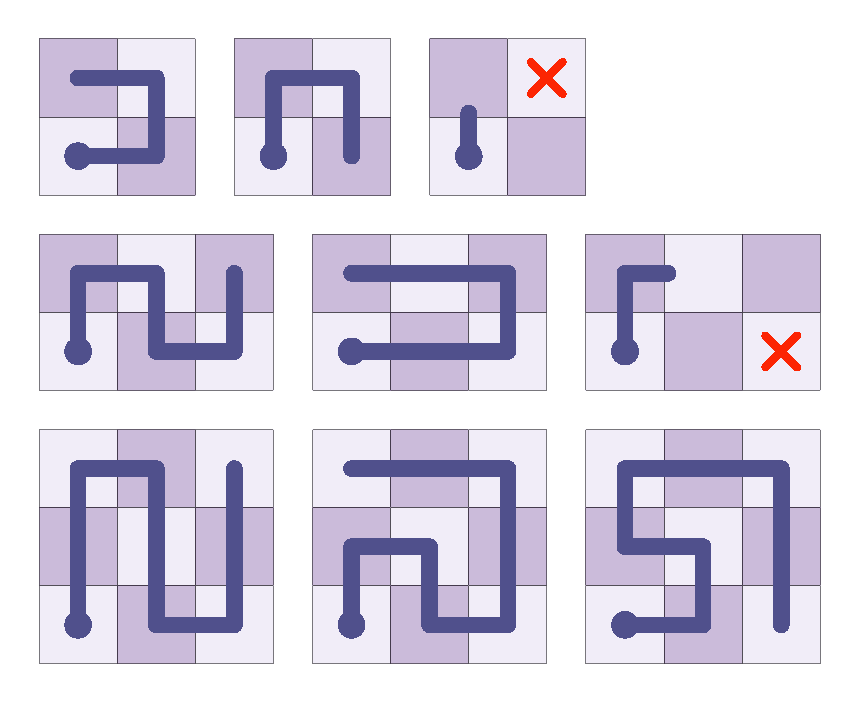
\includegraphics[width=\linewidth]{simple_hampath.pdf}
  \caption{ Illustrative examples of Hamiltonian paths height/width that are even/even, even/odd and odd/odd, respectively,
            when starting from the lower left hand corner }
  \label{fig:exampleHampath}
\end{figure}


The feasibility of determining whether there exists a Hamiltonian path in a rectangular cuboid
grid region can be accomplished through parity arguments.
Label grid cell points in a volume as 0 or 1,
alternating between labels with every axis-aligned single step move.
Any Hamiltonian path that ends at one of the three remaining corners has to have the same parity as the starting point if the
volume is odd, or different parity if the volume is even.

\begin{table}[h]
  \centering
  \begin{tabular}[t]{cr|cc}
    \multicolumn{2}{c}{ \multirow{2}{*}{Path Possible} } & \multicolumn{2}{c}{Volume} \\
    & & \textit{even} & \textit{odd} \\
    \hline
			%\multirow{2}{*}{$|\alpha| \bmod 2$} & \textit{even} & Yes & Yes \\
      \multirow{2}{*}{ $|\alpha|$ } & \textit{even} & Yes & Yes \\
       & \textit{odd} & \textbf{No} & Yes \\
     \hline
  \end{tabular}
  \caption{ Table showing when a Hamiltonian path is possible. Here, $|\alpha|$ is the absolute difference in start and end position of the path which
            coincides with one of the axis aligned side length of the cuboid volume. A Hamiltonian path is possible only when $|\alpha|$ even of both
            $|\alpha|$ and the volume are odd. }
  \label{table:pathTable}
\end{table}


For a path starting at $(0,0,0)$ and ending $|\alpha|$ steps in one of the axis-aligned dimensions,
then Table \ref{table:pathTable} enumerates this condition under which a valid path is possible.
Figure \ref{fig:exampleHampath} illustrates this for starting position $(0,0)$ with volumes $(2 \times 2)$, $(3 \times 2)$ and $(3 \times 3)$,
where a red cross indicating a precluded endpoint.

Without loss of generality, we will assume a curve starts from position $p_s=(0,0,0)$ and has proposed
endpoint at $p_e=((w-1),0,0)$, with a cuboid region as $\alpha = (w,0,0), \beta = (0,h,0), \gamma = (0,0,d)$.
We state, without proof, that
a Hamiltonian path is always possible from $p_s$ to $p_e$ when $|\alpha|$ is even or when $|\alpha|$, $|\beta|$ and $|\gamma|$
are all odd  $(|\alpha| \cdot (1 - |\beta| \cdot |\gamma|) \equiv 0 \bmod 2)$.

With this condition, any cuboid subdivision will always have a Hamiltonian path within it and we can recreate a Hamiltonian
path in the larger cuboid by connecting endpoints from the ending point of one cuboid to the starting point of the succeeding cuboid.
For cuboids that violate this condition, there will be a required notch and
an feasible cuboid subdivision is possible
for all but one of the cuboid subdivisions, recursively limiting the notch violation to a single point.


%%%%%%%%%%%%%%%%%%%%%%%%%%%%%%%%%%%%%%%%%%%%%%%%
%            _ ____              __ ___       __
%     ____ _(_) / /_  ___  _____/ /|__ \ ____/ /
%    / __ `/ / / __ \/ _ \/ ___/ __/_/ // __  / 
%   / /_/ / / / /_/ /  __/ /  / /_/ __// /_/ /  
%   \__, /_/_/_.___/\___/_/   \__/____/\__,_/   
%  /____/                                       
%%%%%%%%%%%%%%%%%%%%%%%%%%%%%%%%%%%%%%%%%%%%%%%%


\subsection{2D Generalized Hilbert Function (Gilbert2D)}

\begin{figure}[h]
  \centering
  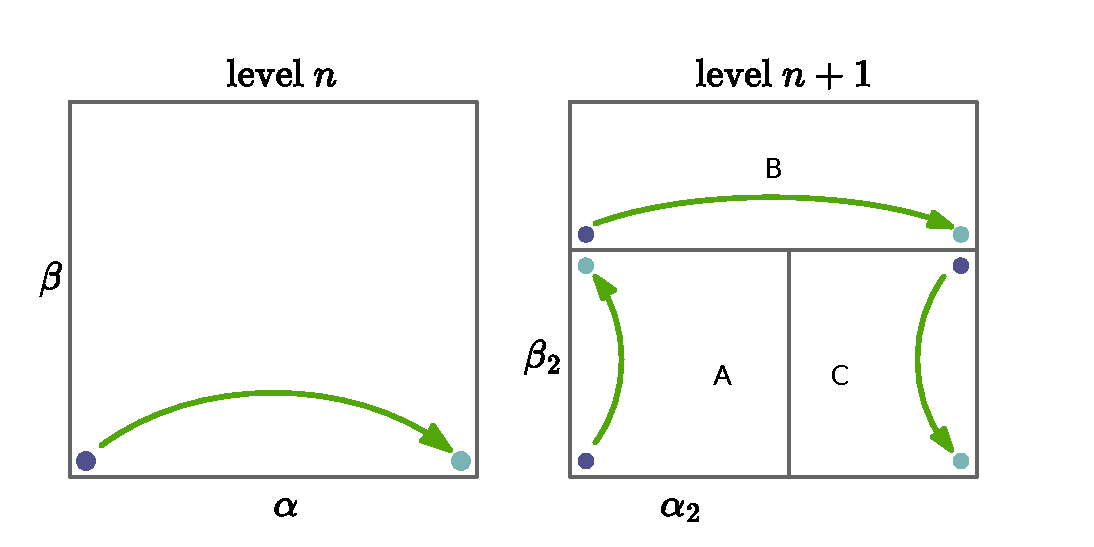
\includegraphics[width=\linewidth]{gilbert2d_mainsubdiv.pdf}
  \caption{ For the 2D Gilbert curve, the main rectangle is subdivided into three sub regions, making sure their paths connect
            and preferring even side lengths for the first rectangular subdivision.
            Partitioning the rectangle in this way is what we call a $U$-split.  }
  \label{fig:main2dsubdiv}
\end{figure}


\begin{figure*}[ht]
  \centering
  \includegraphics[width=\linewidth]{config_production.pdf}
  \caption{ Enumeration of the subdivision template depending on different parities of $\alpha$ and $\beta$ dimensions. }
  \label{fig:production2d}
\end{figure*}

For the 2D Gilbert curve, a $U$-split template is used, highlighted in Figure \ref{fig:main2dsubdiv}.
The $U$-split breaks the region into three sub-blocks, labeled $A$, $B$ and $C$.
Each of the $A$, $B$ and $C$ regions have local coordinate systems that are resized, rotated and
new endpoints chosen so the process can be recursively re-applied.

The sides of the subdivided blocks $A$, $B$ and $C$ are chosen to remain integral.
The width-like dimension for subdivided block $A$ is chosen to be even ($\beta_2$ in Figure \ref{fig:main2dsubdiv})
by dividing the height-like dimension of the original region ($\beta$ in Figure \ref{fig:main2dsubdiv}) by two and by adding one if need be.
Since the width-like length of the subdivided $A$ and $C$ block is even ($\beta_2$), there is a guaranteed valid Hamiltonian path 
in both.

Should the original width-like length be even ($\alpha$ in Figure \ref{fig:main2dsubdiv}), the $C$ block will continue to have 
a valid Hamiltonian path.
If the original width-like dimension is odd, a Hamiltonian path is not possible and there is a forced notch that will appear in the subdivided block $C$.

Figure \ref{fig:production2d} gives examples of the different parity conditions for the original area,
as well as the different conditions when the $A$ and $C$ subdivided areas are coerced into having even parity.
Figure \ref{fig:production2d} also shows when a Hamiltonian
path is not possible, indicated by a red cross, and illustrates how the notch is pushed into the $C$ block
under these conditions.

If a subdivided block becomes too long in its width-like dimension, the block is divided in half and the recursion
proceeds as normal.
Even sides are only enforced if the length is larger than 2, with a length 2 or smaller representing the base
case.
The base case enumerates paths in the axis direction of length greater than one.

% redundant...
Since $A$ and $C$ are chosen to have an even width-like local axis length, no new notches are introduced and any
obligatory notch is effectively ``pushed'' into the $C$ block.


%The $A$ block is chosen to to have a preference for even height dimension


\begin{algorithm}
  \caption{\hskip0.5em 2D Generalized Hilbert Function (Gilbert2D) } %($p$, $\alpha$, $\beta$) \\ \hskip3.0em $p, \alpha, \beta \in \mathbb{Z}^3$ }
  \label{alg:gilbert2d}
  \begin{algorithmic}

    \State \textit{\# $p, \alpha, \beta \in \mathbb{Z}^3$}
    \Function{Gilbert2D}{$p$, $\alpha$, $\beta$}
      \State
      \State $\alpha_2, \beta_2  = \text{div}(\alpha, 2), \text{div}(\beta, 2)$

      \State
      \If{ $(|\beta| \equiv 1)$ }
        \State \textbf{yield} $p + i \cdot \delta(\alpha)$ \textbf{forall} $i \in |\alpha|$

        \State
      \ElsIf{ $(|\alpha| \equiv 1)$ }
        \State \textbf{yield} $p + i \cdot \delta(\alpha)$ \textbf{forall} $i \in |\beta|$

        \State
      \ElsIf{ $(2 |\alpha| > 3 |\beta|)$ }
        \If{ $(|\alpha_2| > 2)$ and $(|\alpha_2| \bmod{2} \equiv 1)$ }
          \State $\alpha_2 \leftarrow \alpha_2 + \delta(\alpha)$
        \EndIf
        \State
        \State \textbf{yield} Gilbert2D($p$, \\ \hskip9.75em $\alpha_2$, $\beta$)
        \State
        \State \textbf{yield} Gilbert2D($p + \alpha_2$, \\ \hskip9.75em $\alpha - \alpha_2$, $\beta$)

        \State
      \Else
        \If{ $(|\beta_2| > 2)$ and $(|\beta_2| \bmod{2} \equiv 1)$ }
          \State $\beta_2 \leftarrow \beta_2 + \delta(\beta)$
        \EndIf
        \State
        \State \textbf{yield} Gilbert2D($p$, \\ \hskip9.75em $\beta_2$, $\alpha_2$)
        \State
        \State \textbf{yield} Gilbert2D($p + \beta_2$, \\ \hskip9.75em $\alpha$, $(\beta - \beta_2)$)
        \State
        \State \textbf{yield} Gilbert2D($p + \alpha - \delta(\alpha) + \beta_2 - \delta(\beta)$, \\ \hskip9.75em $\beta_2$, $-(\alpha - \alpha_2)$)
      \EndIf
    \EndFunction
  \end{algorithmic}
\end{algorithm}

Algorithm \ref{alg:gilbert2d} shows the pseudo-code for computing the 2D Gilbert curve.
Note that $\alpha$ and $\beta$ are taken to be vectors in 3D, where the third dimension
can be ignored if a purely 2D curve is desired.
The generalization to 3D allows the Gilbert2D function to be used unaltered when the
3D Gilbert curve needs to trace out in-plane sub-curves.

The $\delta(\cdot)$ function returns one of the six directional vectors indicating which of
the major signed axis aligned directions the input vector points to ($(\pm1,0,0), (0,\pm1,0),(0,0,\pm1)$).
For completeness, the function is defined in Procedure \ref{alg:delta}.

Algorithm \ref{alg:gilbert2d} assumes standard Euclidean two norm ($|v| = \sqrt{v_0^2 + v_1^2 + v_2^2}$)
and abuses notation by allowing scalar to vector multiplication ($i \in \mathbb{Z}, v \in \mathbb{Z}^3, i \cdot v \to [ i \cdot v_0, i \cdot v_1, i \cdot v_2 ]$).
where the context is clear.

\begin{figure}[h]
  \centering
  \includegraphics[width=\linewidth]{gilbert2d_examples.pdf}
  \caption{ Example outputs of the 2D Gilbert curve algorithm for width and height of i) $8 \times 8$ ii) $18 \times 6$ iii) $13 \times 8$ and iv) $14 \times 14$.
            The $8 \times 8$ Gilbert curve (i) is identical to the Hilbert curve of length $8$.
            For the 13x8 curve (iii), there is no Hamiltonian path possible from $(0,0)$ to $(12,0)$ resulting in the Gilbert curve algorithm inserting a notch
            in the upper right hand corner. }
  \label{fig:gilbert2d_examples}
\end{figure}

Example outputs of the \textit{Gilbert2D} function are listed in Figure \ref{fig:gilbert2d_examples}, showing realizations for dimensions
$(8 \times 8)$, $(18 \times 6)$, $(13 \times 8)$ and $(14 \times 14)$.
The $(8 \times 8)$ (i) in Figure \ref{fig:gilbert2d_examples}) Gilbert curve is identical to the Hilbert curve of side length 8.
The $(18 \times 6)$ (ii) curve highlights a horizontal split when the $\alpha$, or width-like, dimension becomes $\frac{3}{2}$ larger than the
$\beta$, or height-like, dimension.
For the $(13 \times 8)$ (iii) Gilbert curve, a Hamiltonian path is not possible and the algorithm inserts a notch in a best effort approach to realize the curve.

%%%%%%%%%%%%%%%%%%%%%%%%%%%%%%%%%%%%%%%%%%%%%%%%%
%            _ ____              __ _____     __
%     ____ _(_) / /_  ___  _____/ /|__  /____/ /
%    / __ `/ / / __ \/ _ \/ ___/ __//_ </ __  / 
%   / /_/ / / / /_/ /  __/ /  / /____/ / /_/ /  
%   \__, /_/_/_.___/\___/_/   \__/____/\__,_/   
%  /____/                             
%%%%%%%%%%%%%%%%%%%%%%%%%%%%%%%%%%%%%%%%%%%%%%%%%

\subsection{3D Generalized Hilbert Function (Gilbert3D)}


\begin{figure}[h]
  \centering
  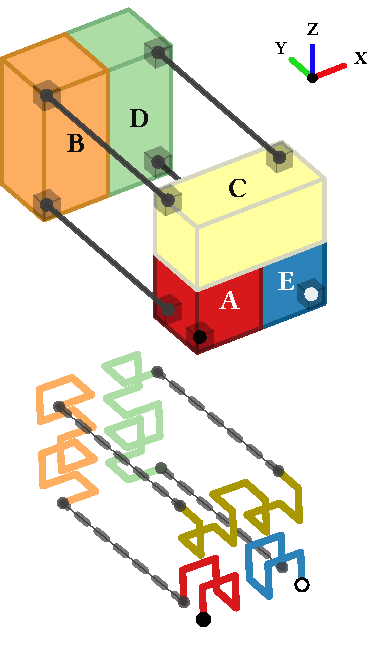
\includegraphics[width=\linewidth]{gilbert3d_explode.pdf}
  \caption{ The $J_0$-split subdivision, representing the main subdivision of the bulk recursion for the 3D Gilbert curve case. }
  \label{fig:gilbert3DJSplit}
\end{figure}


The concept of a $U$-split is extended to 3D by constructing a $J$-split shape templates.
An exploded view of the $J_0$ shape template is shown in Figure \ref{fig:gilbert3DJSplit}.

As discussed in section 3.1, we consider $p \in \mathbb{Z}^3$ to be the local origin point in the cuboid with
$\alpha, \beta, \gamma \in \mathbb{Z}^3$ to be the local basis whose lengths encode the size of the cuboid.
The generalized 3D Hilbert algorithm (\textit{Gilbert3D}) is shown in Algorithm \ref{alg:gilbert3d}.


\begin{algorithm}
  \caption{ \hskip0.5em 3D Generalized Hilbert Function (Gilbert3D) }
  \label{alg:gilbert3d}
  \begin{algorithmic}
    \State \textit{\# $p, \alpha, \beta, \gamma \in \mathbb{Z}^3$}
    \Function{Gilbert3D}{$p$, $\alpha$, $\beta$, $\gamma$}

    \State
    \State\textit{\# Parity of dimensions}

    \State $\alpha_0 \leftarrow (|\alpha|\bmod{2})$
    \State $\beta_0 \leftarrow (|\beta|\bmod{2})$
    \State $\gamma_0 \leftarrow (|\gamma|\bmod{2})$

    \State
    \State\textit{\# Base cases }
    \State \textbf{if} ($(|\alpha|\equiv 2)$ and $(|\beta|\equiv 2)$ and $(|\gamma| \equiv 2)$)
    \State \hskip1.5em \Return Hilbert3D($p$,$\alpha$,$\beta$,$\gamma$) 
    \State \Return Gilbert2D($p$,$\beta$,$\gamma$) \textbf{if} $(|\alpha| \equiv 1)$
    \State \Return Gilbert2D($p$,$\alpha$,$\gamma$) \textbf{if} $(|\beta| \equiv 1)$
    \State \Return Gilbert2D($p$,$\alpha$,$\beta$) \textbf{if} $(|\gamma| \equiv 1)$

    \State
    \State\textit{\# Eccentric cases }

    \State \textbf{if }$(3 |\alpha|>5|\beta|) \text{ and } (3|\alpha|>5|\gamma|))$
    \State \hskip1.5em \Return $S _ 0$($p$,$\alpha$,$\beta$,$\gamma$) 
    \State \textbf{if }$(2 |\beta| > 3 |\gamma|) \text{ or }(2 |\beta| > 3 |\alpha|))$
    \State \hskip1.5em \Return $S _ 2$($p$,$\alpha$,$\beta$,$\gamma$)
    \State \textbf{if }$(2 |\gamma| > 3 |\beta|)$
    \State \hskip1.5em \Return $S _ 1$($p$,$\alpha$,$\beta$,$\gamma$)

    \State
    \State \textit{\# Bulk recursion }
    \State \Return $J _ 0$($p$,$\alpha$,$\beta$,$\gamma$) \textbf{if} $(\gamma_0 \equiv 0)$
    \State \Return $J _ 1$($p$,$\alpha$,$\beta$,$\gamma$) \textbf{if} $(\alpha_0 \equiv 0)$or$(\beta_0\equiv 0)$
    \State \Return $J _ 2$($p$,$\alpha$,$\beta$,$\gamma$)

    \EndFunction

  \end{algorithmic}
\end{algorithm}


Side lengths of the subdivided cuboids are chosen to try and not preclude a
Hamiltonian path, if possible.
If a path starts at the local $(0,0,0)$, a Hamiltonian path that ends
at $((w-1),0,0)$ is only possible when $w$ is even or when all lengths are odd, including $w$.
That is, only when $(|\alpha| \cdot ( 1 - |\beta| \cdot |\gamma| ) \equiv 0 \bmod 2)$ will a Hamiltonian
path be possible through the cuboid region.

Should a Hamiltonian path not be possible, all but one sub-cuboid regions are chosen to allow a Hamiltonian
path.
The sub-cuboid where a Hamiltonian path is not possible will be further subdivided as necessary, recursively
ensuring that the infeasible Hamiltonian path region will eventually be resolved at a single point.

When considering a cuboid region to trace out a Gilbert curve on, there are conceptually three main guides:

\begin{itemize}
  \item \textit{Bulk Recursion Case:} \\ The cuboid region defined by $\alpha, \beta, \gamma$ is sufficiently cube-like
  \item \textit{Eccentric Case:} \\ One of $|\alpha|, |\beta|, |\gamma|$ are significantly larger or smaller than the other two dimension
  \item \textit{Base Case:} \\ One of $|\alpha|, |\beta|, |\gamma|$ are length 1 or all are length 2
\end{itemize}


\begin{figure*}[ht]
  \centering
  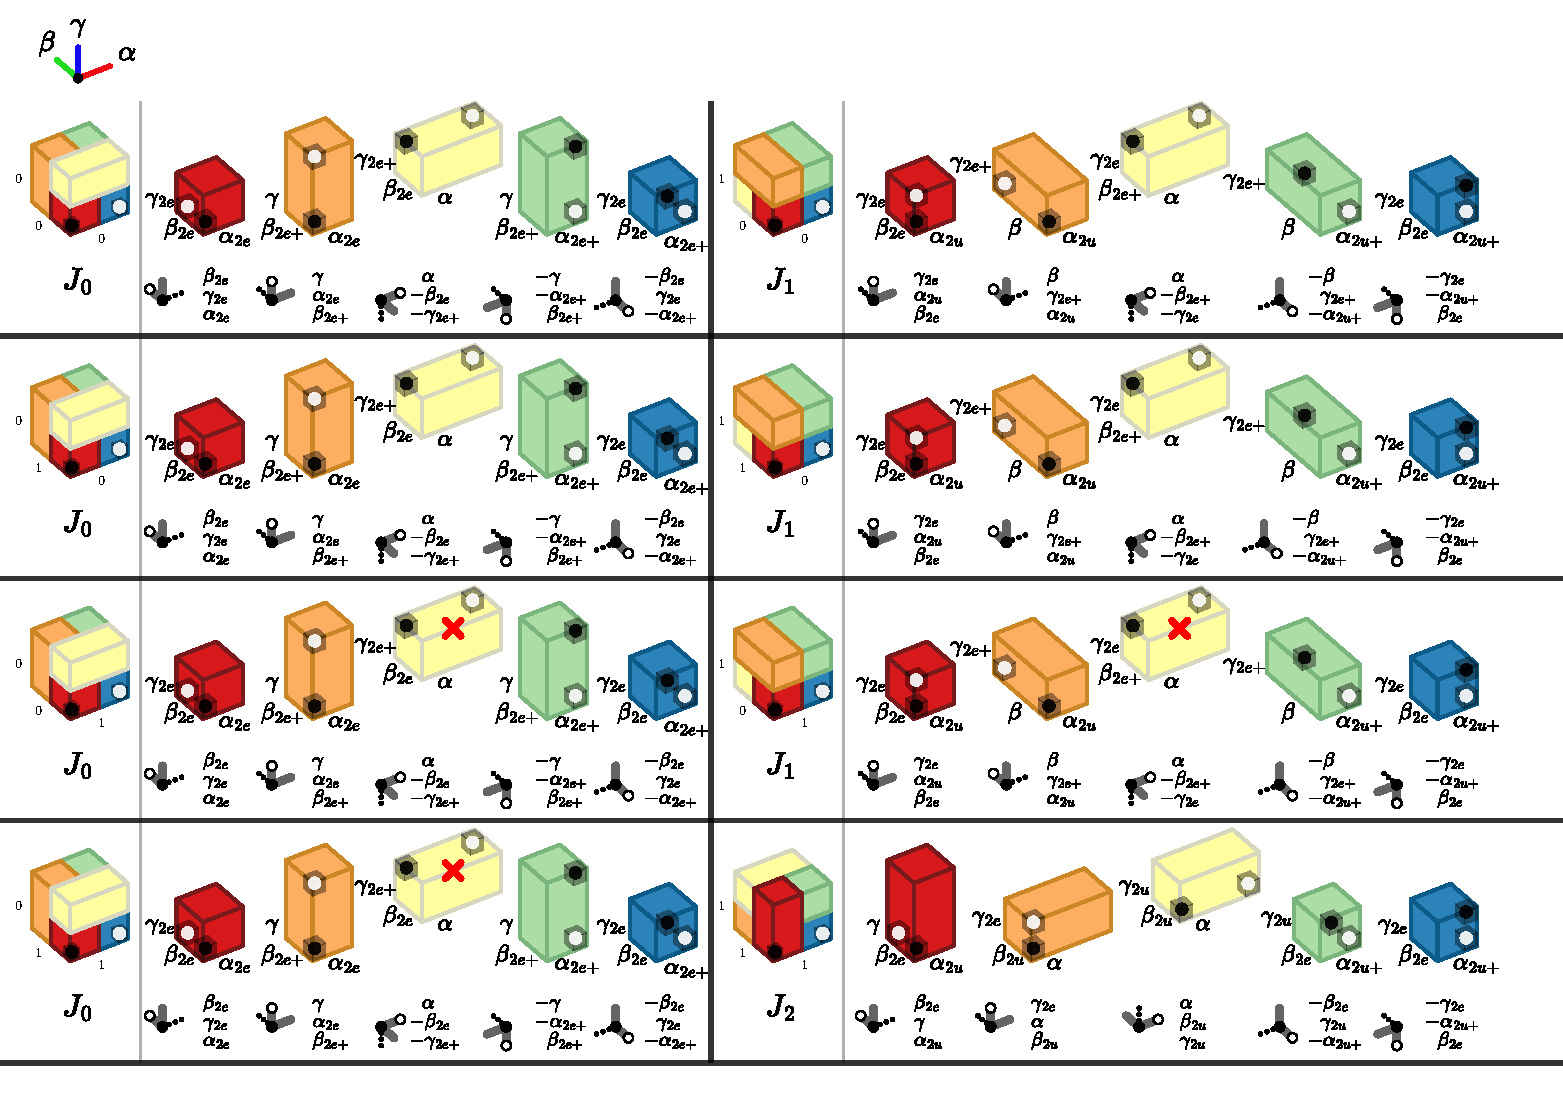
\includegraphics[width=\textwidth]{gilbert3d_case.pdf}
  \caption{ Bulk recursion J-split atlas for the 3D Gilbert algorithm. A subscript of $2e$ is used to denote a preference
  to coerce the length even where as the subscript $2u$ is used to denote a preference to coerce the length odd.
  The subscript $2e+$ is the remainder of the axis after removing the $2e$ portion (e.g. $\alpha_{2e+} = \alpha - \alpha_{2e}$).
  The subscript $2u+$ is the remainder of the axis after removing the $2u$ portion (e.g. $\beta_{2u+} = \beta - \beta_{2u}$).
  The parity of the original cuboid volume are shown in the left most, assembled, volume, for each of the rows.
  The local axis for each of the subdivided cuboid regions is shown underneath them, with a white dot
  denoting the ``width-like'' axis, a solid line denoting the ``height-like'' dimension and a dotted line
  denoting the ``depth-like'' dimension. For each of the cuboids, the block dot denotes the start of the path
  and the white dot denotes the path end. A red cross is used to show when a Hamiltonian path is not possible within a cuboid volume.  }
  \label{fig:gilbert3DCase}
\end{figure*}


For the \textit{bulk recursion case}, there are three main shape templates, $J_0$, $J_1$ and $J_2$.
An atlas of which $J$-split to choose, what parity each of the subdivided cuboid regions and how
to connect each of the subdivisions is shown in Figure \ref{fig:gilbert3DCase}.
Figure \ref{fig:gilbert3DCase} also enumerates the local coordinate system for each of the sub-cuboid
regions, displayed under each of the exploded sub-cuboid region volumes.
When a Hamiltonian path is infeasible,
a red cross is shown on the cuboid region where the notch will be directed to.
Pseudo-code for each of the $J$-split functions is provided in Appendix \ref{JSplitFunctions}

For many of the subdivisions, there is some choice of parity for non-constrained sides.
For example, if all sides start out even (parity $0$), the $J_0$ template would be used, constraining
$\beta_2$ to be even but otherwise allowing $\gamma_2$ and $\beta_2$ to be chosen as even or odd parity.

For conceptual simplicity, $|\beta_2|$ and $|\gamma_2|$ are preferred even.
Should $|\alpha|$ be even, $|\alpha_2|$ is preferred even.
Otherwise, in the case $|\alpha|$ odd, $|\alpha_2|$ is preferred odd.

When $|\alpha|$, $|\beta|$ or $|\gamma|$ become smaller than 2, coercing the respective sub-cuboid
side lengths to be odd or even is not done, as the sub-cuboid region can be safely reduced to its
lower dimensional base case.

The \textit{base case} reduces to \textit{Gilbert2D} if at least one of the dimensions is 1 or a straight forward call to a Hilbert curve
procedure in the case all dimensions have length 2 (\textit{Hilbert2x2x2} in Appendix \ref{AuxiliaryFunctions}).

\begin{figure}[h]
  \centering
  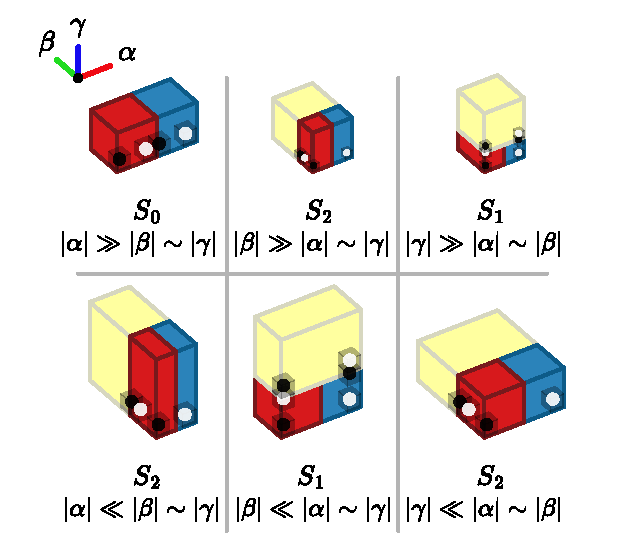
\includegraphics[width=\linewidth]{gilbert3d_eccentric.pdf}
  \caption{ Eccentric cases for recursion. When the cuboid is too far from being cube-like, an $S$-split shape template is used to try and subdivide the cuboids into elements that are more cube like. Here $\alpha$, $\beta$, $\gamma$ are the width-like, height-like and depth-like dimensions. See the text or the algorithm description for the ratios used to determine eccentricity. }
  \label{fig:gilbert3DEccentricCase}
\end{figure}

In the \textit{eccentric case}, where a cuboid region is too lopsided or oblong, an $S$-split is used to try to shape
sub-cuboid regions to be more cube-like.
Figure \ref{fig:gilbert3DEccentricCase} shows the three shape templates, $S_0$, $S_1$, $S_2$, along with the connecting
points, for the different conditions when one axis length is significantly different from the others.
Pseudo-code is provided for each of the $S$-split functions in Appendix \ref{SSplitFunctions}.

When $|\alpha| > \frac{5}{3} \max(|\beta|, |\gamma|)$, the $S_0$ template is used to partition the cuboid the $\alpha$ axis.
In the other cases, when $|\gamma| > \frac{3}{2} \max(|\alpha|, |\beta|)$ or $|\beta| < \frac{2}{3} \min(|\alpha|, |\gamma|)$ the $S_1$
template is used and the $S_2$ template is used when
$|\alpha| < \frac{2}{3} \min(|\beta|, |\gamma|)$,
$|\gamma| < \frac{2}{3} \min(|\alpha|, |\beta|)$ or
$|\beta| > \frac{3}{2} \max(|\alpha|, |\gamma|)$.

\begin{figure*}[ht]
  \centering
  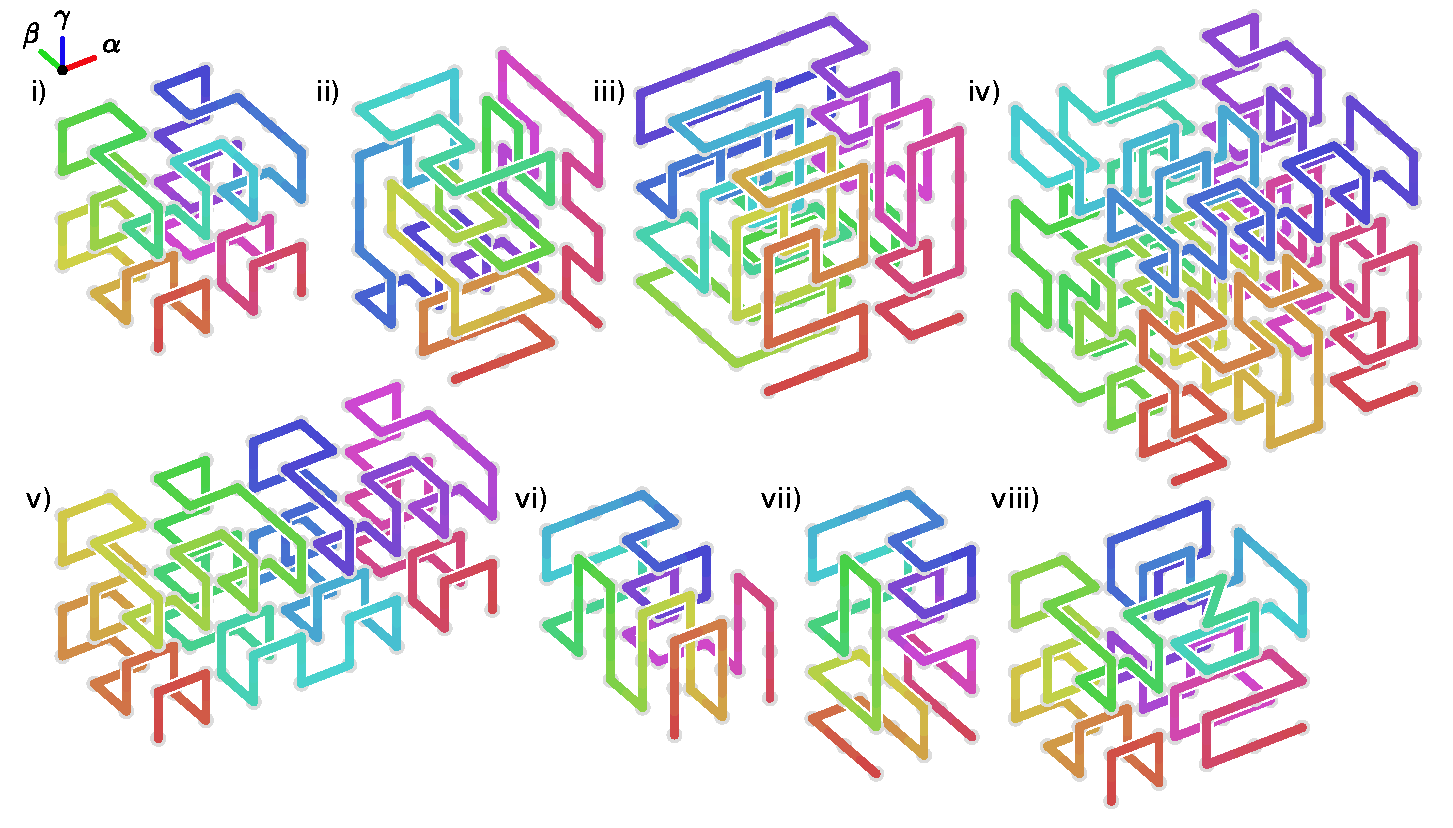
\includegraphics[width=\linewidth]{gilbert3d_examples.pdf}
  \caption{ Examples
  of 3D Gilbert curves highlighting different aspects of the algorithm.
  i) $(4 \times 4 \times 4)$, equivalent to the Hilbert curve of the same side lengths.
  ii) $(4 \times 4 \times 5)$ show a $J_1$ split subdivision scheme.
  iii) $(5 \times 5 \times 5)$, shows a $J_2$ split subdivision scheme.
  iv) $(6 \times 6 \times 6)$, shows a $J_0$ subdivision scheme.
  v) $(8 \times 4 \times 4)$, shows an $S_0$ subdivision scheme, splitting on the $\alpha$ dimension.
  vi) $(3 \times 5 \times 3)$, shows an $S_2$ subdivision scheme.
  vii) $(3 \times 3 \times 5)$, shows an $S_1$ subdivision scheme.
  viii) $(5 \times 4 \times 4)$, shows an example of a configuration where a diagonal move (\textit{notch}) is formed
  as there's no Hamiltonian path possible for the given endpoints.
  }
  \label{fig:examples3d}
\end{figure*}


Figure \ref{fig:examples3d} shows curated example curves for dimensions.
Example \textit{i} shows a Gilbert curve of $(4 \times 4 \times 4)$, reducing to a Hilbert curve of the same dimension.
Examples \textit{ii}, \textit{iii} and \textit{iv} show Gilbert curves of $(4 \times 4 \times 5)$, $(5 \times 5 \times 5)$
and $(6 \times 6 \times 6)$ showing a $J_1$, $J_2$ and $J_0$ split, respectively.
An $S_0$, $S_2$ and $S_1$ split are showing in the \textit{v}, \textit{vi} and \textit{vii} Gilbert curves of
lengths $(8 \times 4 \times 4)$, $(3 \times 5 \times 3)$ and $(3 \times 3 \times 5)$ respectively.
A Gilbert curve with an unavoidable notch is 
shown in \textit{viii}, where the side lengths $(5 \times 4 \times 4)$ preclude a Hamiltonian path from $(0,0,0)$ to $(4,0,0)$.


The constants used to determine eccentricity are chosen by considering the \textit{average defect} of the subdivided cuboid volumes.
We use the term \textit{defect} to mean the ratio of volume of a cuboid region to the cube of its smallest length.
That is:

$$
\begin{array}{l}
  \text{defect}(|\alpha|, |\beta|, |\gamma|) \overset{\mathrm{def}}{=} \frac{ |\alpha| \cdot |\beta| \cdot |\gamma| }{ \min(|\alpha|, |\beta|, |\gamma|) }
\end{array}
$$

For a cube, the defect will be 1, with an increasing defect the larger a side length becomes relative to the other two.

The \textit{average defect} is defined to be the sum of the individual sub-cuboid defect, weighted by each sub-cuboids proportional
volume.

The concept of defect is ad hoc and has potential problems\footnote{For example,
if one dimension is of length 1, the denominator will always be 1.
Further, under this definition, the $J$-split will lead to an increase defect even though another recursion level for a $J$-split on the eccentric
cuboids would lead to a near equal defect, indicating a recursive definition might be better.}.
Regardless, with this ad hoc definition, we can justify constants used for the eccentric cases by showing a defect reduction, relative
to the bulk recursion case.

For the $S_0$ template, the two subdivided cuboids are chosen to be roughly half $|\alpha|$.
For the other templates making the obvious choice of subdividing the ``height-like'' axis by half does
not lead to a defect reduction.
That is, choosing a roughly half subdivision of $|\gamma|$ for $S_1$ or a roughly half subdivision of $|\beta|$ for $S_2$, does
not always yield a defect reduction.

A constant of $\frac{1}{3}$ is chosen to split the ``height-like'' dimensions for the $S_0$ and $S_1$ case,
while the other split is chosen at the halfway mark.
The calculations showing that the constants chosen yield a defect reduction in each of the three eccentric $S$-splits is provided in Appendix \ref{appendix:defect}.

\subsection{Extensions \textbf{d2xyz} and \textbf{xyz2d}}

To provide an index to point lookup or to convert a point to an index along the curve,
Algorithm \ref{alg:gilbert2d} and Algorithm \ref{alg:gilbert3d} can be modified.
Since the recursion is on cuboid regions, we can adjust an index or point easily
by skipping over the appropriate number of cells.

%We use the convetion \textbf{d2xyz} to indicate the index to point lookup function.
A function to convert from an index along the Gilbert curve to a point in space is provided as \textit{Gilbert2D\_d2xyz} in Appendix \ref{alg:gilbert2d_d2xyz}.
A destination and current index is added to the function call, where the destination index is tested
against the current updated index to test whether it should fall into the recursion.
Otherwise, cuboid regions are skipped without processing, providing an $O( \log N )$ worst case run time.

A similar function to convert from a point in space to an index along the curve is called \textit{Gilbert2D\_xyz2d} and is provided in Appendix \ref{alg:gilbert2d_xyz2d}.
\textit{Gilbert2D\_xyz2d} functions similarly to \textit{Gilbert2D\_d2xyz} but instead uses a current test point, $q$, to
test whether the recursion is within the cuboid bounds and, if so, recurs.
As with the \textit{Gilbert2D\_d2xyz}, \textit{Gilbert2D\_xyz2d} provides a worst case execution of
$O( \log N )$ for point to index lookups.

For the sake of brevity, the \textbf{xyz2d} and \textbf{d2xyz} functions are not provided for 3D but the reader is referred to
the reference implementation for details \footnote{ https://github.com/jakubcerveny/gilbert }.

\subsection{Adaptive Extensions}

Applications that require a strict Hamiltonian path without a notch point, but are unconstrained in endpoint location, can choose
endpoints on the even length dimension so that a Gilbert curve with a Hamiltonian path realization is possible.
Other options can include increasing one or more length dimensions with padding to make the major width-like axis ($\alpha$) even or
by forcing all length dimensions to be odd.

\subsection{Corner Cases, Pathological Cases}

For the special case when dimensions are of the form $((2k+1),2)$, for $k \in \mathbb{N}$, the Gilbert curve realization will
not have the ending point of the path at the appropriate location.
For the $((2k+1),2)$ case, no Hamiltonian path is possible from $(0,0)$ to $(2k,0)$ but as an artifact of the algorithm,
a "hook" is formed, causing the last two points to be in different locations.
See Figure \ref{fig:oddxtwo_hook.pdf} for an example configuration.

The hook formed for $((2k+1),2)$ configurations can be removed for a diagonal move by swapping the last two endpoints.
For the sake of clarity and brevity, we leave the algorithm as is, without adding extra complication for this special case.


